The purpose of the evaluation is to assess if a compositional  synthesis of controllers for modular DES plants and LTL goals can perform better than a monolithic approach in which the plant composition is constructed in full. 

For this we implemented compositional synthesis within MTSA~\cite{DIppolito2008}. The only tool we are aware of that is available and \textit{natively} supports controller synthesis for modular DES plants and infinite-trace goals.  By this we mean  means that other tools  do not support describing the system to be controlled as a parallel composition of a set of DES along with some form of specifying  liveness guarantees that are to be achieved. Notably, \cite{supremica} and \cite{eclipse} do modular DES plants, but only allow specifying safety goals. MTSA tool supports GR(1) formulae. We compare MTSA with and without compositional synthesis. 

%\hg{To clarify the scope of the comparison, the reviewers ask the authors to clarify what "native support for modular DES with infinite-trace goals" entails and acknowledge related tools (e.g., Eclipse ESCET/CIF) with a more detailed analysis of their capabilities}

We also study how reactive synthesis tools perform on translated versions of GR(1) DES control problems, both monolithically and compositionally. Specifically, we study  \textit{Spectra}\cite{maoz2021spectra} (a synthesis tool specialized in GR(1)) and Strix\cite{meyer_strix_2018} (a compositional LTL synthesis tool, winner at SyntComp 2023). Note that we did not implement the compositional approach within \textit{Spectra} and \textit{Strix}, rather we had MTSA call them to measure how much time they take to solve the intermediate control problems compositional synthesis necessitates. 

A replication package including tool and control problems is available in \cite{zenodo}.

\subsection{Compositional Synthesis of DES for  GR(1) goals}



Applying the composition synthesis algorithm 
to control problems where $\varphi$ is a GR(1) formula involves three challenges. 
First and foremost, procedures $getLiveController$ and $getSafeController$ must solve control problems that in principle are not GR(1) (i.e., $\Box\Diamond\bigwedge_{l\in \mu}\neg l \implies \varphi$). However, these problems can actually be solved using a GR(1) synthesis algorithm due to the shape of the subplant under analysis  (the only loops consisting of uncontrollable events that can be found in the subplant are in $\mu$ and are self-loops) and the fact that GR(1) formulae are closed under stuttering.
The procedure is to remove in the plant all self-loop transitions labeled with some $l \in \mu \subseteq \Sigma_u$, compute a controller for $\varphi$, and add to the controller the self-loop transitions previously removed to make it legal. This procedure is correct and complete (see proof in Appendix of the technical report submitted in Arxiv).

\begin{theorem}
    \label{lemma:non-flooding-equivalence}
    Given  control problems $\mathcal{E} =  \langle \mathcal{M'} \setminus \{ (s, l, s) \ | \ l \in \mu \cup \mu' \}, \Sigma_c, \varphi \rangle$ and $\mathcal{E'} =  \langle \mathcal{M'}, \Sigma_c, 
     \square \Diamond (\bigwedge_{l \in (\mu \cup \mu')} \neg l)$ $\implies \varphi \rangle$ where $\mathcal{M'} = \mathcal{M} \setminus \{ M_{sub} \} \cup \{ M_{cont} \slash \! \sim_\Upsilon \}$, $\Sigma_c \subseteq \Sigma$ is a set of controllable events, $\mu \ \text{and} \ \mu'$ are sets of events and $M_{cont}$ is a controlled subplant for $\langle \mathcal{M}_{sub}, \Sigma_c, \square \Diamond (\bigwedge_{l \in \mu} \neg l) \implies \varphi\rangle$ where $\mathcal{
     M}_{sub} \subseteq \mathcal{M}$. If there is a solution $C = (S_c, \Sigma, \xrightarrow[]{}_{c}, \hat{s}_c)$ for control problem $\mathcal{E}$, then $C'$ is a solution for $\mathcal{E'}$ where $C' = (S_{c'}, \Sigma, \xrightarrow[]{}_{c'}, \hat{s}_c)$ is defined as follows:
     \begin{itemize}
         \item $S_{C'} = S_C$
         \item $\xrightarrow[]{}_{C'} =  \xrightarrow[]{}_{C} \cup \ \{ (s, l, s) \ | \ s \in S_c \ \wedge \ l \in \Sigma_u \cap (\mu \cup \mu') \ \wedge \ \exists (s_{\mathcal{M'}}, s_{c}) \in S_{\mathcal{M'}||C} \ \cdot \ (\hat{s_{\mathcal{M'}}}, \hat{s_{C}}) \xrightarrow[]{}_{\mathcal{M'}\|C} (s_{\mathcal{M'}}, s_{C}) \ \wedge \ (s_{\mathcal{M'}}, l, s_{\mathcal{M'}}) \in \xrightarrow[]{}_{\mathcal{M'}} \}$. 
     \end{itemize}
     Also, if there is no solution for $\mathcal{E}$ then there is no solution for $\mathcal{E}'$. 
\end{theorem}

A second challenge is an efficient way to compute a safe controller, that is a controller that keeps a plant in states that are non-losing. Furthermore, that the over-approximation of winning states is sufficiently small to achieve state space reductions that make the compositional approach efficient. This can be achieved for GR(1) formulae straightforwardly as the arena for which the underlying game is solved maps back one-to-one to states of the plant. In addition, the GR(1) synthesis procedure\cite{Piterman:2006:SRD} establishes precisely all winning states of the arena. 

Finally, projecting a GR(1) formula to a weaker formula can be done straightforwardly. In our implementation we use the following procedure: For formulae of the form 
 $\varphi = \wedge_{i \in n} \ \always\eventually \phi_i$ $ \implies \wedge_{j \in m} \ \always\eventually \gamma_j$ where $\phi_i$ and $\gamma_j$ are boolean combination of events in conjunctive normal form and $\Sigma' \in \Sigma$ do the following. For every $l \in \Sigma'$, replace every occurrence of $l$ and $\neg l$ with $F$ in every $\phi_i$ and replace every occurrence of $l$ and $\neg l$ with $\top$ in every $\gamma_j$. It is straightforward to see that this projection yields weaker formulae: $\varphi \implies \alpha(\varphi, \Sigma')$.

\subsection{GR(1) DES Synthesis via Reactive Synthesis} 
To study the performance of GR(1) compositional synthesis for DES via reactive synthesis we implemented a translation of MTSA inputs using an approach based on~\cite{majumdar_supervisory_2021}. 
Nonetheless, we developed two different translations.  The first translates each LTS of the plant and also encodes parallel composition rules. We refer to this translation as \textit{modular}.
The second translates the composed plant, a single LTS. We refer to this translation as \textit{non-modular}. Note that the translation is orthogonal to whether monolithic or compositional synthesis will be applied.


For \textit{Strix} we use a binary-encoding for events and local states to reduce the number of atomic propositions needed. Such an encoding is unnecessary for \textit{Spectra} as it supports variables (and performs binary-encoding internally). 

For both \textit{Strix} and \textit{Spectra} we first evaluate how they perform using the modular and non-modular translations for various instances of the benchmark. We then take the best performing translation for each tool to evaluate how a monolithic synthesis approach compares with a compositional one. 

Monolithic synthesis with \textit{Strix} and \textit{Spectra} is achieved by simply translating the plant of the control problem and executing the reactive synthesis tool. 

To avoid modifying \textit{Strix} and \textit{Spectra} to do compositional synthesis, performance is approximated by running a modified version of the compositional MTSA implementation. Every time MTSA calls its internal GR(1) synthesis procedure with a subplant, we mimick the call by calling the synthesis procedure of \textit{Strix} or \textit{Spectra} with a translation of the subplant. The output of reactive synthesis procedure is discarded, and the result of the native GR(1) synthesis procedure is used. We compute the overall time by subtracting the time spent by internal MTSA synthesis procedure. We refer to these approximations of native compositional implementations as \textit{DES Strix} and \textit{DES Spectra}.



\subsection{Benchmark}
 We use modular DES GR(1) control problems taken from multiple sources. Control problems are parameterizable some scale in two dimensions (number of intervening components, $n$, and number of states per component, $k$) and some scale only in the number of intervening components.

For the case studies scalable in two dimensions, we use all problem families introduced in \cite{Ciolek2020}, modified from supervisory control problems to GR(1) control problems: Air Traffic (AT), Bidding Workflow (BW) and Travel Agency (TA), Transfer Line (TL), and Cat and Mouse (CM). We also used a Robot Search Mission (RS) taken from robotic literature \cite{zudaire_assured_2021}.  
All the n-k instances for these problems are known to be realizable, except for those in AT where $n \leq k$ must hold. Thus, we report separately on instances that are realizable (AT$_R$) and those that are not (AT$_{!R}$). We studied for instances with $n, k \leq 9$.

The one-dimension control problems we use are the classic concurrency Dinning Philosophers (DP) problem and the AI planning problem Gripper (GR)~\cite{DBLP:journals/corr/abs-2305-11014}. Finally, we also use a SYNTECH \cite{maoz2021spectra} case study named Moving Obstacle (MO) originally specified as a reactive synthesis problem (i.e., a turn-based game in which each player can update all its variables in each turn).  We translated MO manually into a modular discrete event problem by developing one LTS for each safety property of the specification plus some additional LTS to replicate the turn-based logic of reactive synthesis control. The maximum value for $n$ varies depending on how large the plant for the control problems grows.

Experiments were run on a computer with an Intel i7-7700 CPU @ 3.60GHz, with 8GB of RAM, and a timeout of 30 min. In addition, we use a simple deterministic heuristic for selecting subplants that always chooses the first two LTS from the vector representation of the set $\mathcal{M}$.
% To evaluate the impact of subsystem selection heuristic, we run and compare results for two heuristics: 
% \begin{enumerate}
%     \item Two-Compose, a simple heuristic that composes two by two LTS from automata input set.
%     \item maxS + MaxL \cite{flordal_compositional_2009}, a strategy that select as candidates automatas pairs containing the automaton with the most states and then choose the candidate with the highest proportion of local events.
% \end{enumerate}


% \textbf{Unrealizable ------- }
% \\
% \textbf{Scalable with n, k}
% \begin{itemize}
%     \item AT Congested - Airport unrealizable 
%     \item CM - Cat and Mouse (speedy cat)
%     \item MO - Moving Obstacle (speedy obstacle)
%     \item RS - UAV Robot Search Mission (find person)
% \end{itemize}

\begin{table*}[t]
    \centering
    {
    \scriptsize
    \begin{tabularx}{\textwidth}{|c|c|c|c|c|c|c|c|c|c|c|c|c|c|c|}
        \cline{1-15}
         & Inst. & \multicolumn{2}{c|}{Solved}  & \multicolumn{10}{c|}{Largest instance solved by both Mono and Comp} & State \\ 
         \cline{5-14}

         & & \multicolumn{2}{c|}{Instances}  &  &   & State &  \multicolumn{2}{c|}{Comp Perf.}  & \multicolumn{2}{c|}{Reduction}  & \multicolumn{3}{c|}{Controller} & space\\

         \cline{3-4} \cline{8-14}
         & & Mono & Comp & n & k & space & States & Time & States & Time & LTSs & States & Red. & lgst. inst.\\
      \cline{1-15}
        
        AT$_R$ & 45 & \textbf{35} & 20 & 4 & 4 & $2^{38}$ & 6244 & 110s & -91\% %5.728 
        & -99.63\% %(0.7s)
        & 9 & 6545 & -95.6\%  & $2^{41}$ \\  \cline{1-15}
        % AT_R & 45 & \textbf{35} & 20 & -43\%  & 20  & N=4, K=4 & 5.728 & 0.7s  & 6.244 & 110s  \\  \hline

        AT$_{!R}$ & 36 & \textbf{21} & 15 & 9 & 1 & $2^{42}$ & 17920 & 24s & 33\%  
        & 93\% %(0.7s)
        & -- & -- & --  & $2^{46}$ \\ \cline{1-15}
        
        BW & 81 & 45 & \textbf{50} & 9 & 1 & $2^{22}$ & 1604 & 3s
        & 99.6\% & 96.2\% & 9 & 2499 & 95.6\% & $2^{28}$ \\ 
        \cline{1-15}

        CM & 81 & 20 & \textbf{21} & 4 & 2 & $2^{32}$ & 229993 & 1251s & -51\% & -81.1\% & 7 & 242865 & -91\% & $2^{32}$ \\ 
        \cline{1-15}
        % CM & 81 & 20 & \textbf{21} & 4/2 & 2^{32} & N=4, K=2 & 544.461 & 237s & 229.993 & 1.251s \\ \hline
        
        RS & 81 & 17 & \textbf{29} & 3 & 3 & $2^{24}$ & 24285 & 230s & 90\% & 84\% & 6 & 212664 & 94.3\% & $2^{30}$ \\ 
        \cline{1-15}

        TA & 81 & 50 & \textbf{71} & 6 & 4 & $2^{50}$ & 6560 & 98s &  97.2\% & 93.4\% & 13 & 7951 & 83.3\% & $2^{67}$ \\ \cline{1-15}
        
        TL & 81 & \textbf{30} & 29 & 3 & 6 & $2^{20}$ & 374993 & 231s & -6\% & -49\% & 6 & 377790 & -99.8\% & $2^{20}$\\ 
        \cline{1-15}
        % TL & 81 & \textbf{30} & 29 &  & 29 & N=3, K=6 & 352.940 & 124s & 374.993 & 231s \\ \hline

        %%%%%% 
        % 1V        
        
        DP & 10 & 4 & \textbf{9} & 5 & - & $2^{20}$ & 185 & 1s & 88\% & 96.8\% & 9 & 391 & 97.3\% & $2^{36}$ \\ \cline{1-15}
        % DP & 10 & 4 & \textbf{9} & 125\% & 4 & N=5 & 7.774 & 31s & 185 & 1s \\ \hline

        GR & 20 & 8 & \textbf{11} & 8 & - & $2^{29}$ & 378 & 1s & 99.22\% & 96\% & 17 & 853 & 78\% & $2^{38}$ \\ 
        \cline{1-15}
        % GR & 20 & 8 & \textbf{11} & 8/- & 2^{29} & 8 & N=8 & 48.114 & 24s & 378 & 1s  \\ \hline
        
        MO & 4 & 3 & \textbf{4} & 6 & - & $2^{100}$ & 5180 & 380s & 59\% & 34\% & 38 & 14011 & 44\% & $2^{127}$ \\ \cline{1-15}
        % MO & 4 & 3 & \textbf{4} &  & 3 & N=6 & 12.423 & 472s & 5.180 & 380s \\ \hline

        PC & 10 & 4 & \textbf{10} & 5 & - & $2^{28}$ & 6561 & 220s & 94.8\% & -87\% & 11 & 7152 & 94.3\% & $2^{50}$ \\ \cline{1-15}
        % PC & 10 & 4 & \textbf{10} & 150\% & 4 & N=5 & 124.417 & 30s & 6.561 & 220s \\ \hline
        
        %%%%%% 
        % % NO-V
        % AV & 1 & 1 & 1 & 0 & 1 & - & 45 & 0,047s & 45 & 0,21s \\ \hline
        % PD & 1 & 1 & 1 & 0 & 1 & - & 16 & 0,04s & 39 & 0,06s \\ \hline
        % BO & 1 & 1 & 1 & 0 & 1 & - & 39 & 0,09 & 64 & 0,2s  \\ \hline
        % ME & 1 & 1 & 1 & 0 & 1 & - & ? & ? & 0/1 &  \\ \hline
    \end{tabularx}
    }
    \caption{Experimental Results for Native DES GR(1) Controller Synthesis.}
    \label{table:experimentation}
\label{tab:algorithm_experiment}
\end{table*}
%\vspace{-0.7cm}
\subsection{Results}

\subsubsection{Monolithic vs. Compositional   GR(1) DES Controller Synthesis.} 

%We report on the results of comparing monolithic and compositional synthesis using MTSA. 
Table \ref{table:experimentation} shows results for all case studies.  The first column has problem family names. The next three aggregate information of entire problem families: we show the total number of instances per problem family (Column Inst) and the number of solved instances by the monolithic (Mono) and compositional (Comp) methods. 

These first three columns show that \textit{for 8 out of 10 control problem families, the compositional method improves over the monolithic one} (we count AT$_R$ and AT$_{!R}$ as the same family). 
In all cases the solved instances one of the methods is a superset of the instances solved by the other. 

All problems that the monolithic approach could not solve were due to running out of memory. Also note that providing more RAM to the monolithic method makes little difference in dealing with the combinatorial growth of the state space resulting from increasing the size of problems using $k$ and $n$. Indeed, doubling memory from 8Gb to 16Gb allows the monolithic approach to add less than 5\% more instances. The two problem families in which monolithic performs better than compositional can be explained by looking at the remaining columns.


From the 5th column onwards we focus on the instance with the largest composed plant that was solved by both monolithic and compositional methods. We first report on the values $n$ and $k$ for the instance and its potential state space (i.e., the product of the sizes of all LTS of the plant).
We then report the performance of the compositional method by showing the number of states of the largest plant which the compositional approach solves a control problem for, and the end-to-end time to compute the final controller. The next two columns report the reduction in the largest control problem to be solved with respect to the monolithic method, and the reduction in time to build the final controller compared to the monolothic approach. Negative values in this column indicate that the monolithic approach did better than the compositional.

\textit{For all but three problem families, when considering the largest instance solved by both methods, the compositional approach was able to significantly reduce the plant on which it computes a live controller.} This is an indication of why for these problem families the compositional method has better performance. The exception being 
AT$_!R$ for which, despite achieving reductions, the total number of instances solved by the compositional approach was not greater. This may indicate some bias of our approach towards realizable problems. 

 The three instances for which we report a negative reduction  (AT$_R$($n=4,k=4$), CM($n=4,k=2$), and TL($n=3, k=6$)) show that state explosion of subplants  can  occur and is a likely cause for poor (or in the case of CM, not significantly better) performance of compositional synthesis.


Notice that treating smaller  (sub)plants does not necessarily mean a reduction in time. Instance PC($n=5$) shows that the compositional method is good at reducing size, but a price is paid in time (mostly spent minimizing subplants).  

The next three columns, show the size of the controller computed by the compositional method. We report in column LTSs how many LTSs is the controller composed of. The States column reports the sum of the states of each of these LTS, other words, a measure of the memory required to store the controller on the computer that will enact the controller. We also show the reduction in memory, measured in states, with respect to the (monolithic) controller computed by the monolithic method. \textit{Note that there are significant reductions in the size of the compositional controller for all case studies except for the three in which there are  intermediate state explosions of subplants.}

The final column shows the theoretical size of the biggest instance solved by either of the methods. Subtracting column 7 (``state space'') we obtain how much bigger was the biggest problem solved by one approach than the biggest of the other: For 4 out of 10 problem families, the compositional approach was able to solve instances at least 3 orders of magnitude  ($\times 2^{10}$) bigger than the monolithic approach. For 3 out 10, the increase in size that the compositional algorithm was able to manage was of at least $2^{6}$ larger. On the other hand for the 3 case studies where monolithic fared better, the largest instances it was able to solve were only $2^{6}$ times bigger. 
 


The final column reports on the state space of the largest instance solved, be it the compositional or the monolithic method. For 4 out of 10 case studies, the compositional approach was able to solve instances at least 3 orders of magnitude  ($\times 2^{10}$) bigger than the monolithic approach. For 3 out 10, the increase in size that the compositional algorithm was able to manage was of at least $2^{6}$ larger. On the other hand for the 3 case studies where monolithic fared better, the largest instances it was able to solve were only $2^{6}$ times  bigger. 


The survival plot on the top left of Figure~\ref{fig:cactus-performance} provides a graphical summary of the comparative performance of monolithic vs. compositional GR(1) DES controller synthesis implemented in MTSA. Overall compositional can solve more (and significantly larger) subjects but takes more time than monolithic.

We now discuss possible causes for variable performance of  compositional synthesis across different problem families. We hypothesise that compositional synthesis has opportunities for increased performance when intermediate subsystems can be reduced due to minimization with respect to local events, and when reduction is achieved by reducing reachable states when the subsystem is controlled via partial synthesis.  The main threat to performance is, we believe, having intermediate subsystem state explosion as a result of composing LTS that are very loosely synchronized (worst case being that the composition yields the cartesian product of states). 
Below we analyze two problem families where compositional synthesis performance was worse than monolithic (AT   TL) and one in which it was better (DP). 

For AT, there are two classes of LTS affected by parameters $n$ and $k$: The number of airplane LTS is determined by $n$ and the number of height monitors (that check that at a particular height, there is never more than one airplane)  is determined by $k$. The height monitors interact very little with each other, while each one interacts frequently with all airplanes. Additionally, there is always just one ramp and one response monitor. The response monitor interacts with each airplane on a specific label that is local to that airplane. 

The simple heuristic used composes incrementally height monitors inducing, early on, an intermediate state explosion as their composition yields a state space that is almost the size of the cartesian product of height monitors' states. In addition, there are no local shared events that can lead to intermediate reductions.  
We speculate that a heuristic that starts with the response monitor and adds one airplane at a time will perform better because local shared variables provide opportunities for reduction. Indeed, initial explorations seem to indicate this. 

In instances of TL, there are LTSs representing the machines connected by buffers on a transfer line and an LTS at the end, the Testing Unit (TU), that takes a work piece from the last buffer and accepts it or rejects and returns it to the first buffer for reprocessing.

The naive heuristic we used selects Machines and Buffers in order from the beginning, thus the TU machine is included in the composition towards the end. These intermediate subsystems have permissive controllers because the projected formula (that only talks about events in the TU) is trivial, so they cannot be reduced by partial synthesis. We speculate that a heuristic that starts with TU and adds consecutive machines and buffers from the end towards the beginning of the line will perform better. Initial exploration indicate this is the case. 

In contrast, consider instances of DP, where the compositional approach performs better. The heuristic chooses to add LTSs following the ring architecture defined by the philosophers sitting round the table. Thus, as one more adjacent LTS is added to the subsystem, some new local shared events (between a particular philosopher and a particular fork) can be minimized. Also, since this problem has a formula that refers to events in all philosophers, there are opportunities of minimize by partial synthesis solving control problem for each subsystem.

% Regarding compositional approach performance and specification structure}

% To evaluate the relationship between the performance of our approach and the architecture of the plant, we assess each of the case studies as follows. For each problem family, we analyzed how many pairs of LTSs have at least one local event (i.e., a label that appears in both alphabets but is not present in any others). We expect our minimization algorithm to perform better when applied to subsystems with many local events. Therefore, this is an important aspect to consider when evaluating heuristic decisions.
% Thus, we built a graph representation for each problem family architecture based on this idea. 

% Firstly, we tried to understand why some cases, such as AT and TL, have poor performance with respect to the monolithic approach. We started by analyzing the structure of the AT (whether realizable version or not) case study and noted the existence of two types of LTSs in this architecture: those who belong to a subsystem that shares local variables and those that strictly do not share local variables with any other. The basic heuristic we implemented composes LTSs from both types generating an intermediate state explosion caused by disjoint alphabet between LTSs alphabets.

% On the other hand, we analyze why TL case study has a poor performance when we use compositional approach. After observing the structure, we observed that each LTS is poorly connected with the others (i.e. there are not LTSs sharing local variables). This means that is almost impossible to find a subsystem which has a good performance reducing equivalent states.

% For the DP instance, where the compositional approach performs particularly well in minimizing intermediate results, we identified a ring architecture with a lot of local events in each subsystem which is a great feature for synthesis equivalence algorithm causing a good performance in our approach.

% Also, we can observe a similar behavior for the rest of the cases where our algorithm performs better than monolithic.


\vspace{-0.5cm}
\subsubsection{
Monolithic vs Composition GR(1) synthesis via Reactive Synthesis.}

\textit{Strix} performed consistently better when using the non-modular translation than when using the modular one. This provides some evidence that t\textit{he compositional approach Strix has built in (where smaller problems are solved by selecting subsets of formulae) is not able to exploit the modular nature of the DES control problem. } Results for \textit{Spectra} were opposite. The tool performed consistently better when applied to modular translations of the control problems instead of non-modular ones. 
Thus, for the remaining experiments we used modular translations for \textit{Spectra} and non-modular ones for \textit{Strix}. 


 Top right and bottom left survival plots of Fig. \ref{fig:cactus-performance} show comparative performance of compositional vs monolithic \textit{DES Strix} and \textit{DES Spectra}. 
%Firstly, using MTSA, we observe that the compositional approach solved approximately 5\% more cases than the monolithic one, although it required more time. 
 \textit{DES Strix} solved the same number of cases with both approaches, but the monolithic method took over 50\% more time.
Conversely, bottom left survival plot shows that in \textit{DES Spectra} compositional and monolithic solve the same number of cases, but the monolithic approach is slightly over 20\% faster.

A closer look at \textit{DES Spectra} results reveal that the monolithic tends to perform better on problems with shorter and more centralized formulas (i.e., share alphabet with less LTS).
%On the other hand, monolithic approach uses a modular translation which avoid state-explosion problem of DES representation.
%In contrast, the compositional approach shows advantages on larger, more decentralized specifications, where the modularity helps manage complexity.
By splitting problem families based on whether monolithic or compositional \textit{DES Spectra} does better we can see (bottom right of Fig. \ref{fig:cactus-performance}) that for one set of problem families compositional cumulative time grows much less than that of monolithic, while for the other, compositional cumulative time is higher but grows at a closer rate to that of monolithic. 


% \hg{Texto viejo}
% For each problem family we selected the largest instance that both the compositional MTSA implementation  and either the compositional or monolithic DES version of Strix were able to solve. We used the same criteria for Spectra.

% \textit{In 9 out of 11 instances  compositional DES Strix fared better than monolitic DES Strix.} For only one of the problem families \textit{AT!r}, did the monolithic approach perform (marginally) better. Neither versions of Strix were able to solve instances of the \textit{MO} problem family.
%  \textit{Similarly, for 9 out of 11 problem families, the compositional DES Spectra approach fared better than the monolithic one.} Only for \textit{BW} and \textit{GR}
% did  monolithic synthesis perform over the compositional one. 

% We present detailed performance results in Tables \ref{tab:spectra_comparison} and \ref{tab:strix_comparison} of the appendix. 
% \hg{Fin Texto viejo}

\vspace{-0.5cm}
\begin{figure}[bt]
    \centering
   \centering
  \setlength{\tabcolsep}{2pt} % Reduce column gap
  \renewcommand{\arraystretch}{0.9} % Reduce row gap
  \begin{tabular}{cc}
    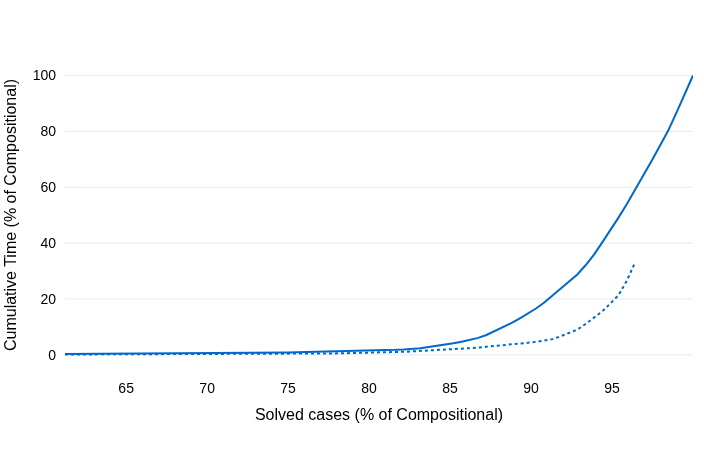
\includegraphics[width=0.4\textwidth]{mtsa_wrtCompositional.png} &
    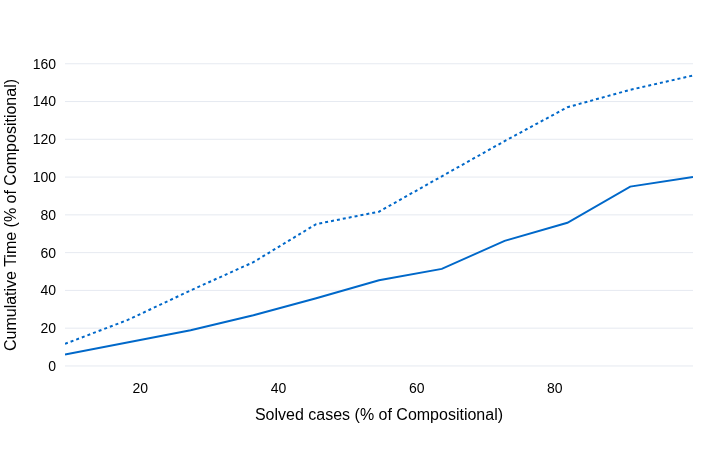
\includegraphics[width=0.4\textwidth]{strix_wrtCompositional.png} 
    \\
    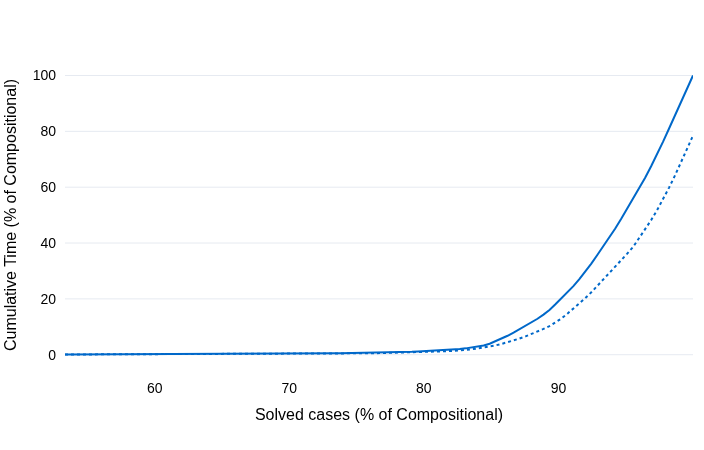
\includegraphics[width=0.4\textwidth]{spectra_wrtCompositional.png} &
    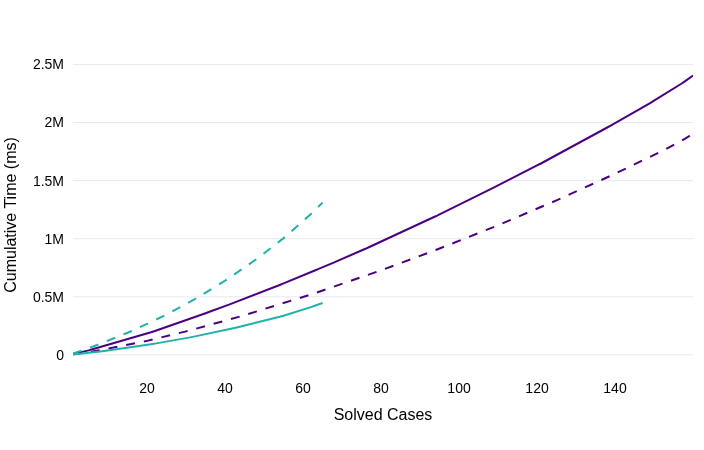
\includegraphics[width=0.4\textwidth]{spectra_differentPerformance.png}
  \end{tabular}
    \caption{Survival plots for Compositional (solid) and Monolithic (dashed) for \textit{DES MTSA} -top left-, \textit{DES Strix} -top right-,  and \textit{DES Spectra} -bottom left-) relative to compositional performance. Bottom right is for \textit{DES Spectra} divided into problem families for which compositional performs better  (purple) and worse (cyan) than monolithic.}
    \label{fig:cactus-performance}
\end{figure}

% \hg{Finally, to better clarify the future potential of the technique, please expand the discussion on when the compositional approach is beneficial vs. when it isn't, especially in relation to the specification structure and plant architecture. Please include a more nuanced analysis of benchmark characteristics that influence performance (e.g., controller pruning effectiveness) and acknowledge explicitly that the currently used heuristics are very basic.}

\subsubsection{Summary.}

The evaluation presented above contributes evidence that compositional synthesis can achieve improvements in scale compared to monolithic DES control, both for native GR(1) DES (explicit state) synthesis, and can achieve improvements in time for DES control via reactive (symbolic state) synthesis. 

For the case of native GR(1) DES synthesis, we observe that performance can degrade if there is intermediate state explosion. Exploring heuristics for choosing subplants that may mitigate this problem. In~\cite{mohajerani_framework_2014} various heuristics are reported to make significant improvements for supervisory control for finite traces. These may also achieve better performance for GR(1) goals.



%% 
% Columna de tamaño teórico

% Dejo solo Tamaño y tiempo de composicional y las del monolítico pasan a ser porcentuales con respccto a composicional.

% Agrego columna con tamaño de C (cantidad de supervisores parciales)
% Agrego columna con la suma de los autómatas de C

%
